\chapter{Badania operacyjne i teoria złożoności obliczeniowej}
\PartialToc




% 1 - 158
\answer
{Która z poniższych złożoności obliczeniowych jest wykładnicza:}
{$O(log 10^n)$}
{F}
{}
{Złożoność obliczeniowa algorytmu jest to ilość zasobów komputera, jakiej potrzebuje dany algorytm. 

Rzędy złożoności obliczeniowej (\textbf{$n$ -- liczba danych wejściowych, $X$ -- stała}):
\begin{enumerate}
\item {Stała -- $O(1)$}
\item {Logarytmiczna -- $O(\log_2(n))$}
\item {Liniowa -- $O(n)$}
\item {Liniowo-logarytmiczna -- $O(n*\log_2(n))$}
\item {Kwadratowa -- $O(n^2)$}
\item {Wielomianowa -- $O(n^X)$}
\item {Wykładnicza -- $O(X^n)$, $O(n!)$}
\end{enumerate}

W powyższym przykładzie $\log 10^n$ jest równoważne $n*\log 10$.
}




% 2 - 159
\answer
{Które z poniższych zdań jest fałszywe:}
{Złożoność czasowa algorytmu pre-order przeszukiwania drzewa jest wielomianowa.}
{?}
{}
{Złożoność czasowa algorytmu pre-order przeszukiwania drzewa jest liniowa. \\

Algorytmy pre-order (prefiksowe), post-order (postfiksowe) i in-order (infiksowe) implementują \textbf{przeszukiwanie w głąb} (Depth First Search -- DFS). Algorytm musi odwiedzić wszystkie wierzchołki ($V$) i wszystkie krawędzie ($E$) drzewa, zatem jego \underline{złożoność czasowa} wynosi $O(|V|+|E|)$.

Złożoność czasowa \textbf{przeszukiwania wszerz} (Breadth First Search -- BFS) wynosi $O(|V|+|E|)$, ponieważ w najgorszym przypadku przeszukiwanie wszerz musi przebyć wszystkie krawędzie prowadzące do wszystkich węzłów.

\underline{Złożoność pamięciowa} przeszukiwania w głąb w przypadku drzewa jest o wiele mniejsza niż przeszukiwania wszerz, gdyż algorytm w każdym momencie wymaga zapamiętania tylko ścieżki od korzenia do bieżącego węzła, podczas gdy przeszukiwanie wszerz wymaga zapamiętywania wszystkich węzłów w danej odległości od korzenia. W tym wypadku złożoność pamięciowa wynosi $O(|V| + |E|)$. \\

\textbf{Binarne drzewo poszukiwań} (ang. Binary Search Tree -- BST) -- dynamiczna struktura danych będąca drzewem binarnym, w którym lewe poddrzewo każdego węzła zawiera wyłącznie elementy o kluczach nie większych niż klucz węzła a prawe poddrzewo zawiera wyłącznie elementy o kluczach nie mniejszych niż klucz węzła. Węzły, oprócz klucza, przechowują wskaźniki na swojego lewego i prawego syna oraz na swojego ojca.

\underline{Koszt wykonania podstawowych operacji} w drzewie BST (wstawienie, wyszukanie, usunięcie węzła) jest proporcjonalny do wysokości drzewa $h$, ponieważ operacje wykonywane są wzdłuż drzewa. Fakt ten w notacji Landaua zapisuje się $O(h)$. Jeżeli drzewo jest zrównoważone, to jego wysokość bliska jest logarytmowi dwójkowemu liczby węzłów ($h \approx \log_2(n)$), zatem dla drzewa o $n$ węzłach optymistyczny koszt każdej z podstawowych operacji wynosi $O(\log n)$. Z drugiej strony drzewo skrajnie niezrównoważone ma wysokość porównywalną z liczbą węzłów (w skrajnym przypadku drzewa zdegenerowanego do listy wartości te są równe: $h=n$), z tego powodu koszt pesymistyczny wzrasta do $O(n)$.
}




% 3 - 160
\answer
{Co przyjmujemy zazwyczaj jako górne ograniczenie w algorytmach podziału i ograniczeń?}
{Wartość funkcji celu najlepszego uzyskanego dotychczas rozwiązania.}
{T}
{}
{Metoda podziału i ograniczeń (ang. B\&B = Branch and Bound) polega na dekompozycji i sterowanym przeszukiwaniu zbioru rozwiązań dopuszczalnych danego problemu. W metodzie podziału i ograniczeń zbiór wszystkich dopuszczalnych rozwiązań danego problemu rozbijany jest na podzbiory. Każdy taki podzbiór odpowiada problemowi o rozmiarze mniejszym niż problem wyjściowy (podproblemowi). 

Rozwiązywany jest on na jeden z następujących sposobów: 
\begin{itemize}
\item poprzez relaksację
\item bezpośrednio
\item pośrednio
\item poprzez podział
\end{itemize}
}



% 4 - 161
\answer
{W algorytmach ewolucyjnych stosowane są różne rodzaje reprodukcji. Która z nich polega na wybieraniu najlepszych osobników z wylosowanych podzbiorów?}
{Reprodukcja proporcjonalna.}
{F}
{Selekcja (reprodukcja) turniejowa.}
{ \\
Rodzaje reprodukcji (preselekcji):

\textbf{Proporcjonalna (ruletkowa)} -- Budujemy wirtualnie koło, którego wycinki odpowiadają poszczególnym osobnikom. Im lepszy osobnik, tym większy wycinek koła zajmuje. Rozmiar wycinków może zależeć od wartości funkcji oceny, jeśli wysoka wartość oceny oznacza wysokie przystosowanie. W takim układzie prawdopodobieństwo, że lepszy osobnik zostanie wybrany jako rodzic, jest większe.

\textbf{Rangowa (rankingowa)} -- obliczamy dla każdego osobnika funkcję oceny i ustawiamy je w szeregu najlepszy-najgorszy. Pierwsi na liście dostają prawo do rozmnażania, a reszta usuwana jest z populacji. Wadą metody jest niewrażliwość na różnice pomiędzy kolejnymi osobnikami w kolejce. Może się okazać, że sąsiadujące na liście rozwiązania mają różne wartości funkcji oceny, ale dostają prawie taką samą ilość potomstwa. Nie posiada wady metody ruletki dotyczącej konieczności skalowania funkcji przystosowania.

\textbf{Turniejowa} -- polega na dzieleniu populacji na grupy i ,,rozgrywaniu turnieju'' pomiędzy osobnikami z poszczególnych grup. Do populacji rodzicielskiej wybierane są najlepsze osobniki z każdej grupy. Selekcji turniejowej można dokonywać w sposób deterministyczny (z prawdopodobieństwem równym 1) lub losowo (p<1). Populację można dzielić na grupy o różnej liczebności (zwykle po 2 lub 3 osobniki). Selekcję turniejową można wykorzystywać w zadaniach optymalizacji wielokryterialnej.

\textbf{Progowa} -- po stworzeniu rankingu powielamy pewną liczbę osobników przekraczających zadany próg, tak aby ich liczba była taka sama jak na początku.

\begin{figure}[h]
\centering
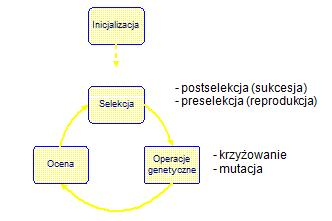
\includegraphics[width=.4\linewidth]{10/algo_ewolucyjne_schemat}
\caption*{Zadanie 10.4: Schemat algorytmów ewolucyjnych}
\end{figure}
}




% 5 - 162
\answer
{Do znalezienia minimalnego czasu wykonania przedsięwzięcia reprezentowanego poprzez graf (sieć) stosuje się metodę ścieżki krytycznej. Na czym polega ta metoda?}
{Na wyznaczeniu najdłuższej ścieżki prowadzącej z wierzchołka początkowego do wierzchołka końcowego.}
{T}
{}
{
Metoda ścieżki krytycznej polega na wyznaczeniu ścieżki w grafie zadań, dla której łączny czas trwania tych zadań jest największy. Czas ten jest minimalnym czasem trwania przedsięwzięcia.

\begin{enumerate}
\item{Najwcześniejszy termin zajścia zdarzenia $j$ oznaczamy przez $t_{j}^w$ i wyznaczamy ze wzoru:\\
$t_1^w = 0 $ : pierwsze zdarzenie może zajść najwcześniej w czasie 0 \\
$t_j^w = max\{t_i^w+t_{i,j}\}$ po $i$ należącym do zbioru wierzchołków, w których rozpoczynają się zadania dochodzące do wierzchołka $j$. $t_j^w$ jest długością najdłuższej ścieżki od wierzchołka 1 do $j$.\\
Czyli zaczynamy od pierwszego wierzchołka i tworzymy najdłuższą ścieżkę.\\
$t_1^w=0, t_2^w=5, t_3^w=10, t_4^w=12, t_s^w=20$}

\item{Najpóźniejszy termin zajścia zdarzenia $i$:\\
$t_s^p = t_s^w$ Ostatnie zdarzenie ma czas wyliczony w punkcie 1\\
$t_i^p = max \{i_j^p - t_{i,j}\}$ po $j$ należącym do zbioru zdarzeń, w których kończą się zadania rozpoczęte z wierzchołka $i$.

Zaczynamy w końcowym wierzchołku, który ma czas wyliczony jako najwcześniejszy termin zajścia zdarzenia w tym węźle, wracamy do wierzchołka startowego i wartość w każdym węźle wynosi (wartość poprzedniego - wartość w ścieżce). W przypadku większej ilości możliwości dojścia do węzła wybieramy tak, by ta wartość była największa. 

\underline{Przykład:} idąc od węzła s do 4 $t_s^p = 20$, $t_4^p = 12$, a z s do 3  $t_s^p = 20$, $t_3^p = 14$. Do węzła 2 możemy dojść przez 3 lub 4, jednak wartość w 2 będzie największa idąc przez 3, więc ten węzeł będzie w ścieżce.
$t_s^p=t_s^w=20, t_4^p=12, t_3^p=14, t_2^p=13, t_1^p=3$}

\begin{figure}[!ht]
\centering
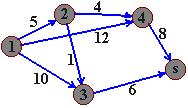
\includegraphics[width=0.5\textwidth]{10/cpm}
\caption*{Zadanie 10.5: Przykład}
\end{figure}

\end{enumerate}
}



% 6 - 163
\answer
{Dla której z podstawowych technik obliczeń ewolucyjnych charakterystyczna jest adaptacja zasięgu mutacji?}
{Dla strategii ewolucyjnych.}
{T}
{}
{ \\
Adaptację zasięgu mutacji stosujemy w strategiach ewolucyjnych, a konkretnie w strategiach $(\mu,\lambda)$ oraz $(\mu+\lambda)$. Strategie $(1+1)$ oraz $(1+\lambda)$ zasięg mutacji określany jest przez dobór odpowiednika współczynnika.
\vspace{0.1cm}

\noindent$\mu$ - populacja rodziców, 
$\lambda$ - populacja potomków
\vspace{0.4cm}

\noindent Inne techniki obliczeń ewolucyjnych:
\begin{itemize}
\item Algorytmy genetyczne
\item Programowanie genetyczne
\item Programowanie ewolucyjne
\item Algorytmy immunogenetyczne
\end{itemize}
}




% 7 - 164
\answer
{Dany jest pierwotny program liniowy postaci:
$c^T x \to max, A \cdot x \leq b, x \geq 0.$
Program dualny do niego ma postać:}
{$b^T y \to max, A^T \cdot y \leq b, y \geq 0.$}
{F}
{$b^T y \to min, A^T \cdot y \geq c, y \geq 0.$}
{
\begin{center}
\begin{tabular}{c | c}
Program pierwotny  & Program dualny       \\ 
\hline \hline
$c^Tx \to max$     & $b^T y \to min$      \\
$A \cdot x \leq b$ & $A^T \cdot y \geq c$ \\
$x \geq 0$         & $y \geq 0$           \\ 
\hline
$c^Tx \to min$     & $b^T y \to max$      \\
$A \cdot x \geq b$ & $A^T \cdot y \leq c$ \\
$x \leq 0$         & $y \leq 0$           \\
\end{tabular}
\end{center}

\begin{itemize}
\item $A$ -- macierz $M\times N$ współczynników stojących po lewej stronie układu warunków ograniczających (czyli mamy $M$ warunków ograniczających i $N$ zmiennych decyzyjnych)
\item $b$ -- wektor kolumnowy $M$ wyrazów wolnych układu warunków ograniczających 
\item $c^T$ -- wektor wierszowy $N$ współczynników funkcji celu
\item $x$ -- wektor kolumnowy $N$ zmiennych decyzyjnych zagadnienia pierwotnego
\item $y$ -- $M$-elementowy wektor kolumnowy nowych zmiennych decyzyjnych (zmiennych dualnych).
\end{itemize}

Program dualny do standardowego zagadnienia maksymalizacji jest standardowym zagadnieniem minimalizacji, zaś program dualny do standardowego zagadnienia minimalizacji jest standardowym zagadnieniem maksymalizacji (czyli jak maksymalizujemy program pierwotny to minimalizujemy program dualny, jak minimalizujemy program pierwotny to maksymalizujemy program dualny).

Charakterystyczne dla programu dualnego jest to, że ma tyle warunków ograniczających, ile zmiennych miał program pierwotny, zaś zmiennych ma tyle, ile warunków miał program pierwotny. Dalej, w programie dualnym wagami funkcji celu są wyrazy wolne zagadnienia pierwotnego, zaś wyrazami wolnymi są wagi funkcji celu programu pierwotnego. Te własności programu dualnego sprawiają, że może być atrakcyjny dla decydenta. Mianowicie, pierwotny problem decyzyjny może mieć liczne zmienne decyzyjne, ale niewielką liczbę warunków ograniczających, zatem program dualny będzie mieć liczne warunki ograniczające, ale niewielką liczbę zmiennych decyzyjnych, przez co może być łatwiejszy do rozwiązania. I gdy istnieje związek (przejście) między rozwiązaniami programów pierwotnego i dualnego, to korzyść z posiadania programu dualnego jest oczywista.
}




% 8 - 165
\answer
{Co nazywamy mostem grafu?}
{Minimalną liczbę krawędzi grafu, których usunięcie zmienia graf w niespójny lub trywialny.}
{F}
{\textbf{(Możliwe dwie)} 
\begin{enumerate}[label=(\alph*)]
\item \textbf{Krawędź grafu spójnego której usunięcie z grafu zmienia go w graf niespójny lub trywialny.}
\item \textbf{Krawędź, której usunięcie spowoduje wzrost liczby składowych spójności grafu.}
\end{enumerate}
}
{Patrz punkt \textbf{10.9}.}




% 9 - 166
\answer
{Jak nazywamy podzbiór $V' \subset V$ zbioru wierzchołków grafu $G = (V, E)$, taki, że każdy węzeł nienależący do $V'$ jest sąsiedni do pewnego elementu z $V'$?}
{Zbiór niezależny.}
{F}
{\textit{To wygląda na pytanie typu ,,odrzuć odpowiedzi, które na pewno nie są prawidłowe'' -- np. znasz pojęcie zbioru niezależnego i wiesz, że to nie to}}
{ 
\begin{itemize}
\item \textbf{Zbiór niezależny} -- zbiór takich wierzchołków w grafie, pomiędzy którymi nie ma żadnej krawędzi
\item \textbf{Podgraf} -- graf uzyskany poprzez usunięcie części wierzchołków wraz z kończącymi się w nich krawędziami
\item \textbf{Graf spójny} –- dla każdej pary wierzchołków istnieje ścieżka, która je łączy
\item \textbf{Graf niespójny} -- graf nieposiadający powyższej własności
\item \textbf{Graf trywialny} -- graf składający się tylko z jednego wierzchołka
\item \textbf{Spójna składowa grafu} -- taki podgraf, który można ,,wydzielić'' z całego grafu bez usuwania krawędzi; graf spójny ma jedną spójną składową
\item \textbf{Graf acykliczny} -- graf niezawierający drogi zamkniętej
\item \textbf{Drzewo} -- spójny, nieskierowany graf acykliczny
\item \textbf{Drzewo spinające grafu} -- spójny, acykliczny podgraf danego grafu, zawierający wszystkie wierzchołki
\item \textbf{Graf pełny} -- wszystkie wierzchołki są ze sobą bezpośrednio połączone
\item \textbf{Klika} -- podgraf pełny
\end{itemize}
}




% 10 - 167
\answer
{Jak nazywamy system obsługi zadań, w którym każde zadanie musi przejść przez wszystkie maszyny w jednakowym, ściśle określonym porządku?}
{System otwarty.}
{F}
{System przepływowy.}
{ \\
W przypadku maszyn dedykowanych rozróżniane są następujące systemy obsługi zadań:
\begin{itemize}
\item \textbf{przepływowy (flow-shop)} -- każde zadanie musi przejść przez wszystkie maszyny w ściśle określonym porządku (każde zadanie składa się zatem z $m$ operacji)
\item \textbf{ogólny / gniazdowy (job-shop)} -- kolejność maszyn mających wykonać operacje jest różna, ale ściśle określona dla każdego zadania (zadania mogą mieć różną ilość operacji)
\item \textbf{otwarty (open-shop)} -- w systemie otwartym wytworzenie każdego wyrobu wymaga operacji na wszystkich maszynach, ale kolejność ich wykonywania jest dowolna i nieustalona.
\end{itemize}
}




% 11 - 168
\answer
{W algorytmie symulowanego wyżarzania z sąsiedztwa bieżącego rozwiązania bazowego losuje się jedno rozwiązanie. Co się dzieje, jeżeli jest ono gorsze od dotychczasowego rozwiązania bazowego?}
{Zastępuje bieżące rozwiązanie bazowe, jeżeli parametr zwany temperaturą jest mniejszy od zera.}
{F}
{Znalezione rozwiązanie zastępuje poprzednie z pewnym prawdopodobieństwem zależnym m.in. od współczynnika nazywanego temperaturą. Temperatura zmniejsza się wraz z kolejnymi iteracjami, co pociąga za sobą spadek prawdopodobieństwa wybrania gorszego rozwiązania.}
{ \\
Termin wyżarzanie pochodzi z metalurgii i dotyczy termodynamicznego procesu studzenia. Jeżeli płynna stal jest schładzana wystarczająco wolno, to ma tendencję do krzepnięcia w strukturze o minimalnej energii. Metoda symulowanego wyżarzania opiera się na analogii do tego procesu. Jej celem jest wyprowadzenie trajektorii poszukiwań z ekstremum lokalnego lub uniknięcie takiego ekstremum. W metodzie tej, z sąsiedztwa aktualnego rozwiązania nie jest wyszukiwane najlepsze rozwiązanie, tylko wybiera się rozwiązanie w sposób losowy. Jeżeli to wylosowane rozwiązanie jest lepsze od bieżącego, to staje się ono nowym rozwiązaniem. W przeciwnym przypadku znalezione rozwiązanie zastępuje poprzednie z pewnym prawdopodobieństwem zależnym m.in. od temperatury. 

Temperatura jest zmieniana w czasie iteracji według tzw. schematu chłodzenia. Im wyższa, tym prawdopodobieństwo wyboru gorszego rozwiązania jest większe. Im niższa, tym algorytm jest bardziej zbliżony w działaniu do typowych metod iteracyjnych. To właśnie znajduje odzwierciedlenie w drugim ważnym aspekcie algorytmu symulowanego wyżarzania czyli w powolnym ochładzaniu.

Na początku działania algorytmu temperatura jest wysoka, dzięki czemu algorytm może bardzo często zmieniać konfigurację rozwiązania, niejednokrotnie wybierając rozwiązanie gorsze. Wraz z kolejnymi iteracjami algorytmu temperatura spada i wybierane są częściej rozwiązania lepsze. Pod koniec pracy algorytmu, temperatura jest na tyle niska, że prawdopodobieństwo wyboru gorszego rozwiązania jest bliskie zeru. Algorytm zachowuje się wówczas, jak typowy algorytm iteracyjny i stara się maksymalnie ulepszyć rozwiązanie.
}




% 12 - 169
\answer
{W teorii złożoności wszystkie problemy decyzyjne, które w wielomianowym czasie rozwiązuje niedeterministyczna maszyna Turinga, tworzą pewną klasę problemów. Jak brzmi jej nazwa?}
{Klasa NP.}
{T}
{}
{ \\
\textbf{Klasa P} --  wszystkie problemy decyzyjne, które w co najwyżej wielomianowym czasie rozwiązuje deterministyczna maszyna Turinga

\textbf{Klasa NP} -- wszystkie problemy decyzyjne, które w co najwyżej wielomianowym czasie rozwiązuje niedeterministyczna maszyna Turinga 

P $\subset$ NP 

Mówimy, że problem decyzyjny $\Pi_1$ jest NP-zupełny, jeśli $\Pi_1 \in$ NP i dla każdego innego problemu decyzyjnego $\Pi_2$  NP zachodzi: $\Pi_2$  $\Pi_1$.

Dla wykazania trudności rozważanego problemu \underline{optymalizacyjnego} (tzn. problemu w którym należy ekstremalizować pewną funkcję celu) wystarcza wykazanie NP-zupełności odpowiadającego mu problemu \underline{decyzyjnego} (tzn. problemu na który odpowiadamy tak lub nie). Mówimy wtedy, że dany problem optymalizacyjny jest \textbf{NP-trudny}.
}





% 13 - 170
\answer
{Zastosowanie metody programu dualnego pozwala na:}
{Zamianę problemu optymalizacyjnego na równoważny -- decyzyjny.}
{F}
{Zamianę problemu pierwotnego -- który posiada liczne zmienne decyzyjne, ale niewielką liczbę warunków ograniczających -- na program dualny, który będzie mieć liczne warunki ograniczające, ale niewielką liczbę zmiennych decyzyjnych, przez co może być łatwiejszy do rozwiązania.
}
{ Patrz punkt \textbf{10.7}.
}




% 14 - 171
\answer
{Dane są algorytmy A i B o złożonościach odpowiednio $O_A(n^3)$ i $O_B((\log n)^3)$. Oba algorytmy wywołano dla pewnych danych wejściowych: $a$ (dla A) i $b$ (dla B). Szybciej (w sensie czasu mierzonego w sekundach) wykona się algorytm:}
{B}
{T}
{}
{Algorytm B ma złożoność logarytmiczną.

\begin{figure}[!ht]
\centering
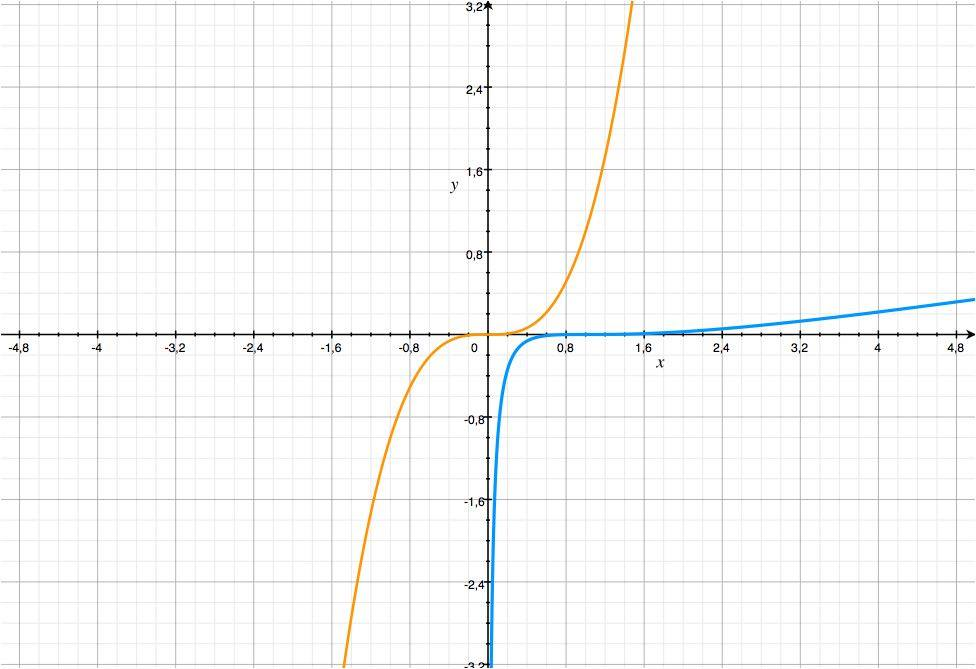
\includegraphics[width=\textwidth]{10/10-4-2}
\caption*{Zadanie 10.14: Oś X to rozmiar danych wejściowych, oś Y to czas obliczeń. Mamy dodatkowo założenie, że X > 1. Widać, że wykresy się ładnie rozmijają i niezależnie od rozmiaru danych wejściowych czas obliczeń jest zawsze mniejszy dla złożoności $(\log x)^3$. Jeżeli wykresy by się przecinały, to znaczy że można znaleźć taki rozmiar danych wejściowych $a$ i $b$.}
\end{figure}
}




% 15 - 172
\answer
{W jakim celu w algorytmach ewolucyjnych stosuje się funkcję kary?}
{Zmniejszenia liczby osobników w populacji.}
{F}
{Funkcję kary stosuje się przy osobnikach reprezentujących niedopuszczalne rozwiązanie. Spowoduje ona dużo mniejsze prawdopodobieństwo przejścia selekcji przez danego osobnika. W zależności od tego, czy funkcję dopasowania minimalizujemy czy maksymalizujemy, wartość funkcji błędu należy do niej dodać bądź odjąć.}
{}
